\documentclass[conference]{IEEEtran}
% *** GRAPHICS RELATED PACKAGES ***
%
\ifCLASSINFOpdf
  \usepackage[pdftex]{graphicx}
  % declare the path(s) where your graphic files are
  % \graphicspath{{../pdf/}{../jpeg/}}
  % and their extensions so you won't have to specify these with
  % every instance of \includegraphics
  \DeclareGraphicsExtensions{.pdf,.jpeg,.png}
\else
  % or other class option (dvipsone, dvipdf, if not using dvips). graphicx
  % will default to the driver specified in the system graphics.cfg if no
  % driver is specified.
  \usepackage[dvips]{graphicx}
  % declare the path(s) where your graphic files are
  % \graphicspath{{../eps/}}
  % and their extensions so you won't have to specify these with
  % every instance of \includegraphics
  % \DeclareGraphicsExtensions{.eps}
\fi

\usepackage{pgf}
%\usepackage{tikz}
%\usetikzlibrary{arrows,automata}

\definecolor{darkgreen}{rgb}{0,0.7,0}

\newif\ifdraft
\drafttrue
%\draftfalse
\ifdraft
 \newcommand{\katznote}[1]{ {\textcolor{blue} { ***Dan:   #1 }}}
 \newcommand{\ketanote}[1]{{\textcolor{orange}  { ***Ketan:   #1 }}}
 \newcommand{\kriedernote}[1]{ {\textcolor{darkgreen}  { ***Scott:   #1 }}}
 \newcommand{\note}[1]{ {\textcolor{red}    {\bf #1 }}}
\else
 \newcommand{\katznote}[1]{}
 \newcommand{\kriedernote}[1]{}
 \newcommand{\note}[1]{}
\fi
% correct bad hyphenation here
%\hyphenation{op-tical net-works semi-conduc-tor}

\hyphenation{Queuing}

\begin{document}
%
% can use linebreaks \\ within to get better formatting as desired
\title{Early Experiences in Running Many-Task Computing Workloads on GPGPUs}

%\author{\IEEEauthorblockN{Auth1\IEEEauthorrefmark{1},
%Auth2\IEEEauthorrefmark{1}\IEEEauthorrefmark{1}, 
%Auth3\IEEEauthorrefmark{1},
%\IEEEauthorblockA{\IEEEauthorrefmark{1}Argonne National Laboratory}
%}}

\author{Scott J. Krieder\IEEEauthorrefmark{1},
Benjamin Grimmer\IEEEauthorrefmark{1},
Ioan Raicu\IEEEauthorrefmark{1}\IEEEauthorrefmark{2}\\
\IEEEauthorblockA{
\IEEEauthorrefmark{1}Department of Computer Science, Illinois Institute of Technology}
\IEEEauthorrefmark{2}MCS Division, Argonne National Laboratory
}


\maketitle


\begin{abstract}
This work aims to enable Swift to efficiently use accelerators (such as NVIDIA GPUs) to further accelerate a wide range of applications. This work presents preliminary results in the costs associated with managing and launching concurrent kernels on NVIDIA Kepler GPUs. We expect our results to be applicable to several XSEDE resources, such as Forge, Keeneland, and Lonestar, where currently Swift can only use the general processors to execute workloads and the GPUs are left idle.
\end{abstract}

% no keywords
\begin{IEEEkeywords}
Many-Task Computing, Swift, GPGPU, CUDA
\end{IEEEkeywords}

\IEEEpeerreviewmaketitle

\section{Introduction}
Many-task computing (MTC) \cite{raicu2008toward} aims to bridge the gap between two computing paradigms, high throughput computing (HTC) and high-performance computing (HPC). MTC emphasizes using many computing resources over short periods of time to accomplish many computational tasks (i.e. including both dependent and independent tasks), where the primary metrics are measured in seconds. MTC denotes high-performance computations comprising multiple distinct activities, coupled via file system operations. Swift is a particular implementation of the MTC paradigm, and is a parallel programming system that has been successfully used in many large-scale computing applications across the TeraGrid and now XSEDE. \cite{zhao2007swift} Swift has been adopted by the scientific community as a great way to increase productivity in running complex applications via a dataflow driven programming model, which intrinsically allows implicit parallelism to be harnessed based on data access patterns and dependencies. Swift has been shown to run well on tens of thousands of nodes with task graphs in the range of hundreds of thousands of tasks. This work aims to enable Swift to efficiently use accelerators (such as NVIDIA GPUs and Intel Xeon Phi \cite{Xeon_Phi_web}) to further accelerate a wide range of applications. This work evaluates a real biochemistry application, namely the Open Protein Simulator (OOPS) \cite{OOPS}, which builds on the Protein Library (PL). OOPS is multipurpose and allows extensions to perform various simulation tasks relevant for life scientists, such as protein folding or protein structure prediction. We have taken parts of this application and ported to NVIDIA GPUs via the CUDA programming language, in order to accelerate OOPS computations via Swift. This work presents preliminary results in the costs associated with managing and launching concurrent kernels on NVIDIA FERMI GPUs, through the Swift system. We expect that our results to be applicable to several XSEDE resources, such as Forge, Keeneland, and Lonestar, where currently Swift can only use the general processors to execute workloads and the GPUs are left idle.

\section{Many-Task Computing and Swift}
Many-task computing (MTC) aims to bridge the gap between two computing paradigms, high throughput computing (HTC) and high-performance computing (HPC). MTC emphasizes using many computing resources over short periods of time to accomplish many computational tasks (i.e. including both dependent and independent tasks), where the primary metrics are measured in seconds. MTC denotes high-performance computations comprising multiple distinct activities. Swift is a particular implementation of the MTC paradigm, and is a parallel programming system that has been successfully used in many large-scale computing applications across the TeraGrid and now XSEDE. It has been adopted by the scientific community as a great way to increase productivity in running complex applications via a dataflow driven programming model, which intrinsically allows implicit parallelism to be harnessed based on data access patterns and dependencies.

\section{Accelerators and Coprocessors}
There are currently three major players in the hardware accelerator market including NVIDIA GPUs, AMD GPUs \cite{AMD_web}, and the Intel Xeon Phi. Running CUDA on NVIDIA GPUs is one of the most mature GPGPU solutions and provides high raw computational performance, however this does require code ported to the CUDA platform. The Intel Xeon Phi suffers from a lack of availability, but once this device is highly available it should bring large improvements in regards to accelerator programmability due to the familiar x86 environment. Finally, AMD GPUs provide a high level of openness in regards to programmability. AMD supports open standards such as OpenCL but may see difficulty in adoption within the HPC markets due to performance.\cite{kriederGCASR12}

\section{Architecture and Evaluation}
Without a scheduler, jobs run on the GPU following the pattern copy-compute-copy as shown in Figure \ref{fig:no_scheduler}. In addition, copy-compute-copy produces inefficiencies some of which are shown in the red area of Figure \ref{fig:red}. Our scheduler sits in-between Swift and GPU. Handles multiple inputs from Swift and condenses these into single GPU calls. Use of a scheduler allows for overlapping kernel execution. Finally, our scheduler overlaps data transfers from the last solution and next problem to increase efficiency.


\begin{figure}[h]
\centering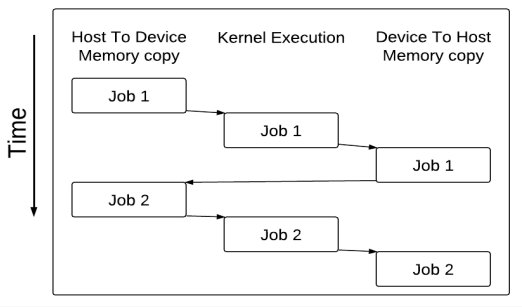
\includegraphics[width=8cm]{imgs/no_scheduler.png}
\caption{By default jobs on the GPU run pattern copy-compute-copy.}
\label{fig:no_scheduler}
\end{figure}

\begin{figure}[h]
\centering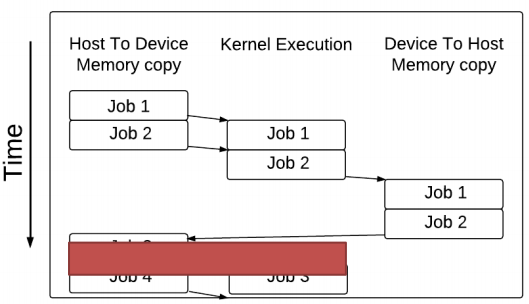
\includegraphics[width=8cm]{imgs/red.png}
\caption{Inefficiencies of copy-compute-copy highlighted in red.}
\label{fig:red}
\end{figure}

Our current implementation is a static batch FIFO scheduler. Sleep jobs demonstrate our schedulers ability to overlap kernels as shown in Figure \ref{fig:sleep}. Finally, with PCI-e 2 we are able to complete copies in just a few microseconds as shown in Figure \ref{fig:comm}. This leads us to believe a SuperKernel managed MTC scheduler will not bottleneck on mem copies.

\begin{figure}[h]
\centering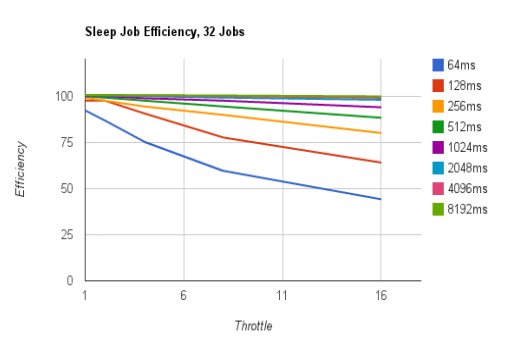
\includegraphics[width=8cm]{imgs/sleep.png}
\caption{Inefficiencies of copy-compute-copy highlighted in red.}
\label{fig:sleep}
\end{figure}

\begin{figure}[h]
\centering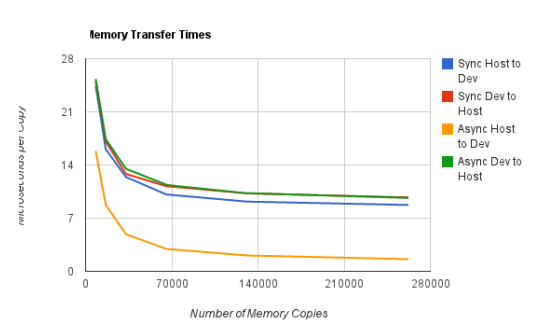
\includegraphics[width=8cm]{imgs/comm.png}
\caption{Inefficiencies of copy-compute-copy highlighted in red.}
\label{fig:comm}
\end{figure}


\section{Conclusion and Future Work}
Future work aims to migrate our scheduler into the GPU, allowing a daemon SuperKernel to manage the MicroKernels, through the use of CUDA concurrent kernels. We also expect our performance to increase on the latest NVIDIA Kepler Architecture. \cite{NVIDIA_Kepler} By integrating our GPGPU MTC Scheduler into Swift we will be able to provide GPU support for MTC applications that utilize Swift. In addition this will apply the dataflow model to GPUs and provide implicit parallelism at the task level. Finally, we believe that the Intel Xeon Phi will provide an array of added benefits for running MTC workloads. Future work will examine how Intel Xeon Phi performs for MTC workflows.

In conclusion this work presented a scheduler which provides concurrent kernel execution from built in library of CUDA kernels. This scheduler overlaps memory transfers for increased performance. The scheduler supports concurrent kernels limited only by CUDA constraints up to 16 kernels. Finally, our scheduler eliminates Kernel execution overheads and enables workloads with coarse granular kernels.

\bibliographystyle{IEEEtran}
\bibliography{ref}
\end{document}
